
%% LyX 2.1.4 created this file.  For more info, see http://www.lyx.org/.
%% Do not edit unless you really know what you are doing.
\documentclass[oneside,spanish,letterpaper]{book}
\usepackage[T1]{fontenc}
\usepackage[utf8]{inputenc}

       %\usepackage{bickham}
        %\usepackage{boondox-cal}
        %\usepackage{boondox-calo}
       % \usepackage{dutchcal}
       % \usepackage{eulervm} 

\setcounter{secnumdepth}{3}
\setcounter{tocdepth}{3}
\usepackage[spanish]{babel}
\addto\shorthandsspanish{\spanishdeactivate{~<>.}}
\addto\captionsspanish{\renewcommand{\chaptername}{Unidad}}
\renewcommand\spanishtablename{Tabla}

\usepackage{csquotes}
\usepackage{amsfonts}
\usepackage{amssymb}
\usepackage{amsmath}
%%\usepackage[pagebackref,ocgcolorlinks,pdfborderstyle=U]{hyperref}

\usepackage{graphicx}
\usepackage{commath}

\usepackage{esdiff}

\usepackage{mathrsfs}

\usepackage{lipsum}
\usepackage[backend=biber]{biblatex}
\addbibresource{EDA-biblio.bib}

%https://en.wikibooks.org/wiki/LaTeX/Floats,_Figures_and_Captions
%It's possible to get a thin border around all figures.
%You have to write the following once at the beginning of the document:
\usepackage{float}
\floatstyle{boxed} 
\restylefloat{figure}
%ya estaba \usepackage{graphicx}


\newtheorem{ejemplo}{Ejemplo}[section]
\newtheorem{teorema}{Teorema}[section]
\newtheorem{definition}{Definición}[section]
\newtheorem{solution}{Solución}[ejemplo]
\newtheorem{practica}{Práctica}[section]


\newcommand{\sen}{\operatorname{\sen}}

\usepackage{enumitem}
\usepackage{listings}

%\usepackage{breqn}   No usar, rompe la ejecución

\usepackage{hyperref}

\begin{document}

\title{Física General}

\author{Oscar Rendón Aldaraca}

\maketitle

\tableofcontents
%\listoffigures
%\listoftables
\section{Caracterización de la asignatura}
La Física es una ciencia que proporciona al estudiante una presentación clara y lógica de los conceptos y principios básicos, los cuales permiten entender el comportamiento de fenómenos de la naturaleza, y con ello, fortalecer la comprensión de los diversos conceptos a través de una amplia gama de interesantes aplicaciones al mundo real.
La disposición de éstos objetivos hace hincapié en las situaciones con argumentos físicos sólidos. Al mismo tiempo, se motiva la atención del estudiante a través de ejemplos prácticos para demostrarle las formas de aplicar la Física en otras disciplinas, como circuitos eléctricos, aplicaciones electrónicos, etc.; además, coadyuva en el análisis y razonamiento crítico que debe privar en todo ingeniero para la resolución de problemas que se le presenten durante su quehacer profesional.
El ingeniero en Sistemas Computacionales tendrá las herramientas necesarias para poder interactuar con profesionales en otros campos del saber, para que de ésta manera solucione problemas con bases cimentadas en la Física y poder afrontar los retos actuales del desarrollo tecnológico.
\section{Intención didáctica.}
Se organiza el temario en 7 unidades, con los conceptos básicos de la Física en la primera unidad, permite que el estudiante interprete el manejo vectorial de las fuerzas, así como la resolución de problemas de equilibrio, involucrando las ecuaciones básicas de equilibrio, momentos y sus aplicaciones.
En la segunda unidad se hace una revisión del movimiento de los cuerpos clasificando y diferenciando lo que es velocidad, rapidez y aceleración en ejemplos prácticos de la partícula. Y la cinética permite conocer las causas que ocasiona el movimiento y las que se oponen a éste.
La tercera unidad da una visión al estudiante sobre los conceptos de óptica geométrica y sus aplicaciones en el mundo que lo rodea.
En la cuarta unidad se estudian las leyes de la termodinámica, buscando una visión de conjunto de éste campo de estudio. Al hacer una revisión de éstas leyes, se incluyen los conceptos involucrados. La segunda ley es esencial para fundamentar una visión de economía energética.
El estudio y la aplicación de fenómenos electrostáticos se encuentra en la quinta unidad, donde se diferencía el concepto de campo eléctrico y las leyes electrostáticas que rigen este campo. También, permite conocer el potencial eléctrico que generan las cargas electrostáticas, involucrándose con el mundo real.
Además, se presenta la importancia del concepto dieléctrico para que el estudiante observe como puede aumentar o disminuir la influencia de éste en un capacitor, teniendo la oportunidad de interactuar los capacitores con circuitos serie-paralelo, mediante prácticas de laboratorio, con el fin de demostrar la energía almacenada en los capacitores.
La sexta unidad, permite al estudiante conocer el flujo de electrones a través de conductores, identificando el efecto Joule en éstos, debido al paso de la corriente y la integración de circuitos serie-paralelos y estructuración de redes complejas, que le permitan desarrollar los conocimientos elementales de física en aplicaciones prácticas.
Mediante la séptima unidad de este curso, el estudiante conoce la interacción de fuerzas magnéticas entre corrientes eléctricas y campos magnéticos, las leyes que rigen los campos magnéticos y las leyes de generación de la fuerza electromecánica, así como la inductancia magnética.
Es importante la realización de las prácticas propuestas y desarrollar cada uno de los experimentos, para así, hacer más significativo y efectivo el aprendizaje. Algunas de las actividades sugeridas pueden hacerse como actividad extra clase y comenzar el tratamiento en clase a partir de la discusión de los resultados de las observaciones de los experimentos realizados.
En el transcurso de las actividades programadas es significativo que el estudiante aprenda a valorar las actividades que lleva a cabo y esté conciente que está construyendo su hacer futuro y en consecuencia actúe de una manera profesional; así mismo, aprecie la importancia del conocimiento y los hábitos de trabajo; desarrolle la precisión y la curiosidad, la puntualidad, el entusiasmo y el interés, la tenacidad, la flexibilidad y la autonomía. Es ineludible que el profesor ponga atención y cuidado en estos aspectos en el desarrollo de las actividades de aprendizaje de esta asignatura.


\chapter{Estática de la partícula.}
La mecánica se puede definir como la ciencia de la física que describe y predice las condiciones de reposo y movimiento de los cuerpos bajo la acción de fuerzas. Se divide en 3 partes: La mecánica de los cuerpos rígidos, la mecánica de los cuerpos deformables y la mecánica de fluidos. La mecánica de los cuerpos rígidos se subdivide a la vez en estática y dinámica. En esta primera unidad veremos la estática, esto es la mecánica de los cuerpos rígidos en reposo.
\section{Conceptos básicos y definiciones}
El estudio de la mecánica se remonta a los tiempos de Aristóteles (384-322 aC) y a los tiempos de Arquímides (287-212 aC.) sin embargo no es sino hasta Newton que se tuvo una formulación satisfactoria de sus principios fundamentales. Los cuales fueron expresados de forma modificada por D'Alembert, Lagrange y Hamilton. Su validez se mantuvo hasta que Einstein formuló su teoría de la relatividad en 1905. Aunque la mecánica newtoniana tiene sus limitaciones, aún es la base de las actuales ciencias de la ingeniería.\\
Los conceptos básicos que se emplean en la mecánica son el espacio, fuerza, tiempo y masa. Estos conceptos no pueden ser definidos en forma exacta pero deben de aceptarse con base en nuestra intuición y experiencia. El espacio se mide con respecto a un punto de referencia y con 3 longitudes y 3 direcciones. Estas longitudes se conocen como coordenadas de $P$.\\
Para definir un evento no basta con indicar su posición en el espacio sino que debe darse también el tiempo del evento.\\
\paragraph{El concepto de masa} es la cantidad de materia de un cuerpo y si 2 cuerpos tienen la misma cantidad de materia entonces recibirán la misma fuerza de atracción de la tierra y también presentarán la misma resistencia a un cambio de su movimiento translasional.

\paragraph{Una fuerza} representa la acción de un cuerpo sobre otro y puede ejercerse por contacto real o a distancia como las fuerzas gravitacionales y magnéticas. Una fuerza se caracteriza por su punto de aplicación, magnitud y dirección y se representa por lo tanto con un vector, Ver $\mathbf{a}$ en la figura \ref{vector}, que viene a ser la flecha negra (vector $\mathbf{a}$) con punto de aplicación, magnitud y dirección que se ven en el diagrama como las coordenadas $(0,0,0), |\mathbf{a}|$, y la dirección de $\mathbf{a}$ (dirección hacia donde apunta la flecha o sea desde el origen $(0,0,0)$ hasta la punta de la flecha).
\begin{figure}[h]
  \centering\label{vector}
      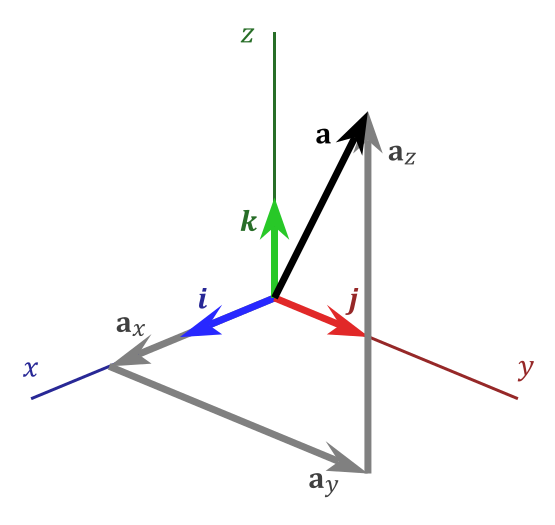
\includegraphics[width=0.5\textwidth]{3D_Vector}
  \caption{Vector. \url{https://upload.wikimedia.org/wikipedia/commons/f/fd/3D_Vector.svg}}
\end{figure}

\paragraph{Un cuerpo rígido}  son muchas partículas con posiciones fijas entre sí.

\paragraph{Ley del paralelogramo para la adición de fuerzas}
2 fuerzas que actúan sobre una partícula pueden ser substituidas por una sola fuerza que es la suma de los vectores (fuerzas), la suma vectorial se hace sobre sus correspondientes dimensiones (coordenadas) por lo que se forma en un campo de 2 dimensiones un paralelogramo y en 3 o más un paralepípedo o hiperparalepípedo, ver figura \ref{paralepiped}, siendo el resultado la conexión entre el origen y el vértice más lejano.
\begin{figure}[h]
  \centering
      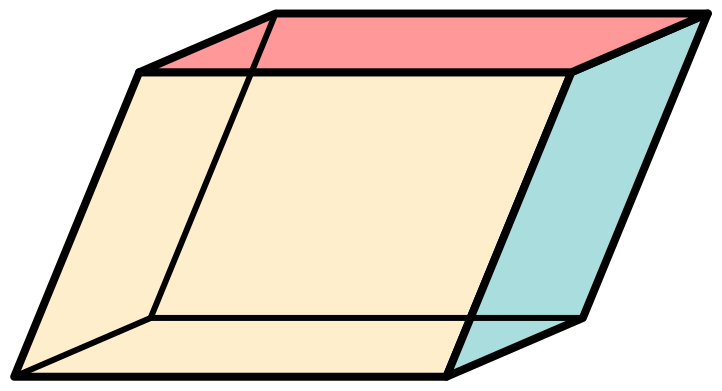
\includegraphics[width=0.5\textwidth]{Parallelepiped_2013-11-29}
  \caption{Paralepípedo. \url{https://en.wikipedia.org/wiki/File:Parallelepiped_2013-11-29.svg}}\label{paralepiped}
\end{figure}
\paragraph{El principio de transmisibilidad} establece que las condiciones de equilibrio o movimiento de un cuerpo rígido permanecerán constantes si una fuerza que actúa sobre el cuerpo rígido se sustituye por otra fuerza de igual magnitud y dirección pero actuando en un punto diferente siempre que las dos fuerzas tengan la misma línea de acción.
\paragraph{Las tres leyes fundamentales de Newton} fueron formuladas por Sir Isaac Newton a finales del siglo XVII y son:
\begin{enumerate}
 \item \textbf{Inercia} si la fuerza resultante de una aplicación de fuerzas a una partícula es 0, entonces la partícula no cambiara su reposo o movimiento. Ver \ref{unaNew}
 \item \textbf{Fuerza} si la fuerza resultante de una aplicación de fuerzas a una partícula no es 0, entonces habrá un cambio en el movimiento o reposo de la partícula proporcional a la magnitud de la fuerza ($|\mathbf{F}|$)\hspace{6pt}\footnote{Los vectores se representarán en negritas. En este caso son vectores de 3 componentes.}
 $$
 \mathbf{F}=m\mathbf{a}
 $$
 \item \textbf{Reacción}, a toda acción corresponde una reacción (fuerza) de la misma magnitud, punto de aplicación y dirección pero de sentido opuesto. 
\end{enumerate}
\paragraph{La ley de gravitación de Newton.} Establece que dos partículas de masa $m$ y $M$ se atraen mutuamente con fuerzas iguales y opuestas $\mathbf{F}$ y $-\mathbf{F}$ de magnitud $F=|\mathbf{F}|$ dada por la fórmula:
\begin{equation}
 F=G\frac{mM}{r^2}\label{fgrav}
\end{equation}

 
 donde $r$= la distancia entre las 2 partículas y $G$= la constante de gravitación
 Una unidad importante es el peso de las cosas $\mathbf{W}$ que viene a ser la fuerza de atracción de la Tierra o cualquier objeto de suficiente tamaño y masa en las cosas de la que se hable. Entonces al dividir la $\mathbf{F}$ entre la masa $m$ del objeto específico tendremos la aceleración de la Tierra sobre ese objeto ya que fuerza es igual a masa por aceleración $(\vec g)=\mathbf{F}/m$ lo que nos dará una atracción hacia el centroide gravitacional del objeto (en este caso la tierra) y cuya magnitud $g$ será:
\begin{equation}
  g=F/m=G\frac{mM}{mr^2}=G\frac{M}{r^2}\label{accg}
\end{equation}

 donde $r$ es la distancia del objeto hasta el centroide gravitacional o de masa del objeto por lo que para la superficie de la Tierra $g$ es $9.81 m/s^2$ \cite{beer-static}
 

\section{Resultante de fuerzas coplanares}
Las fuerzas coplanares son las que están en un mismo plano. Cuando las fuerzas se unen en un mismo punto se tiene una fuerza resultante que se puede calcular en un campo con solo sumar cada componente de las fuerzas por los correspondientes lográndose una fuerza resultante. Cuando los componentes están en un mismo plano se pueden graficar cada par de fuerzas originales generando un paralelogramo ver figura \ref{sVectoresP}. 
\begin{figure}[h]
  \centering\label{sVectoresP}
      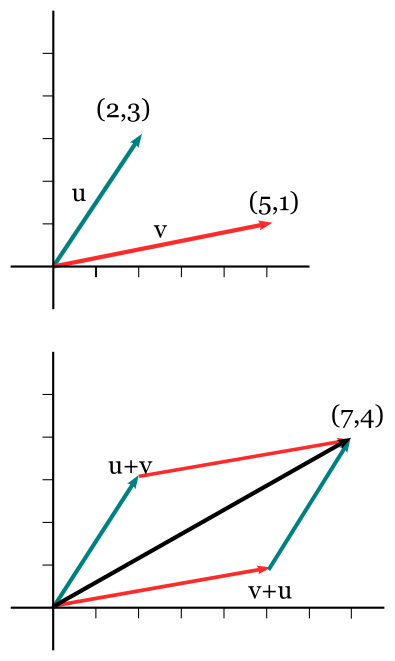
\includegraphics[width=0.5\textwidth]{Suma_de_vectores}
  \caption{Suma de vectores coplanares (Los vectores pueden representar fuerzas, pero muchos otros fenómenos también). \url{https://es.m.wikipedia.org/wiki/Archivo:Suma_de_vectores.svg}}
\end{figure}
Entonces en un plano $\vec{a}+\vec{b}=(a_1,a_2)+(b_1,b_2)=(a_1+b_1,a_2+b_2)$
\begin{enumerate}
 \item $(5,3)N+(2,5)N=$
 \item $(-5,3)N+(2,5)Kgf=$
 \item $(7,3)N+(2,2)N=$
 \item $(14,3)N+(-2,-5)N=$
 \item $(3,3)N+(12,-5)N=$
 \item $(5,3)N+(2,5)N=$
 \item $(-5,-3)N+(3,5)N=$
 \item $(1.5,\pi)N+(-e,5)N=$
 \item $(-2/3,3)N+(a,4)N=$
 \item $(2,x)N+(3,5x)N=$
 \end{enumerate}


\section{Componentes rectangulares de una fuerza}
Una fuerza se considera un vector en un campo euclidiano de 3 dimensiones. O sea la norma o distancia de separación entre 2 puntos de ese campo está dado por:
\begin{equation}
 |\vec{p}-\vec{q}|=\sqrt{\sum_{i=1}^3(p_i-q_i)^2}
\end{equation}
como los 3 ejes en el campo espacial están perfectamente perpendiculares, todas las fuerzas tienen un valor en en cada uno de esos ejes y cuya magnitud está por lo tanto perpendicular a los demás y a lo largo del eje correspondiente. Ésto es un vector fuerza se puede descomponer en sus 3 componentes que serán perpendiculares entre sí (rectangulares o sea en ángulo recto entre sí). Ver figura \ref{vector}. 

\section{Condiciones de equilibrio, primera Ley de Newton}\label{unaNew}
Cuando la suma de las fuerzas es cero en los 3 componentes se dice que las fuerzas están en equilibrio y por lo tanto no hay aceleración ni frenado en el cuerpo que recibe las fuerzas. Dar cada alumno 2 ejemplos de fuerzas en equilibrio. Una en movimiento y otra estática en su marco referencial. 
\section{Cuerpos rígidos y principio de transmisibilidad}\label{transm}
Si se está empujando un auto con una fuerza de 1000 newtons en una superficie horizontal, una fuerza de 1000 newtons que lo jale en la misma direcció mantendrá la misma velocidad que la fuerza que lo empujaba inicialmente. Igual un objeto sostenido en el aire con una mano usará la misma fuerza para ser sostenido que si el mismo objeto es sostenido con una cuerda y la mano, despreciando el peso de la cuerda.
\section{Momento de una fuerza respecto a un punto}
El momento de una fuerza $\mathbf {F} \,\,$ aplicada en un punto P con respecto de un punto O viene dado por el producto vectorial del vector  $ {\overrightarrow {\text{OP}}}\,$ por el vector fuerza; esto es,

 $\mathbf {M} _{\text{O}}={\overrightarrow {\text{OP}}}\times \mathbf {F} =\mathbf {r} \times \mathbf {F} \,$\\
Donde  $\mathbf {r} $ es el vector que va desde O a P. Por la propia definición del producto vectorial, el momento $ \mathbf {M} \,$ es un vector perpendicular al plano determinado por los vectores $ \mathbf {F}\,$ y $ \mathbf {r}$.

El término momento se aplica a otras magnitudes vectoriales como el momento lineal y/o cantidad de movimiento $ \mathbf {p} \,$, y el momento angular o cinético, $ \mathbf {L} \,$, definido como

$ \mathbf {L} _{\text{O}}={\overrightarrow {\text{OP}}}\times \mathbf {p} =\mathbf {r} \times \mathbf {p} $

El momento de fuerza conduce a los conceptos de par, par de fuerzas, par motor, etc.
El producto vectorial se calcula mediante la determinante del vector base unitario y los 2 vectores a los que se les calcula el producto vectorial, esto es la magnitud del área del paralelogramo formado entre los vectores dados, con dirección a la ortogonal al plano entre los mismos, o en otras palabras al producto de sus componentes intercalados en dirección intercalada (ortogonal al plano entre ellos):
\begin{equation}
 \mathbf{A}\times\mathbf{B}=
 \left|
 \begin{array}{ccc}
  \hat{\imath} & \hat{\jmath} & \hat{k}\\
 A_1 & A_2 & A_3\\
 B_1 & B_2 & B_3
 \end{array}
 \right|
\end{equation}
Por lo mismo el momento se puede expresar como el producto de sus magnitudes ortogonales  y cumple la regla de la mano derecha (ver también figura):
\begin{equation}
{\overrightarrow {\text{OP}}}\times \mathbf {F} =|\mathbf {r}|| \mathbf {F}|\sen(\theta) 
\end{equation}

\begin{figure}[h]
  \centering
      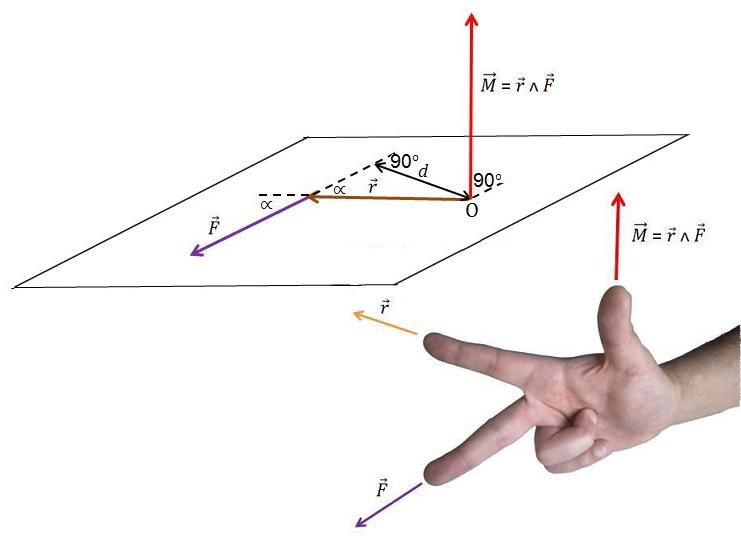
\includegraphics[width=0.5\textwidth]{regla-mano-derecha-sentido-fuerza}
  \caption{El momento cumple lar regla de la mano derecha}\label{MomManDer}
\end{figure}
\cite{wmomento,momentof,beer-static}

\section{Teorema de Varignon}
\begin{teorema}[Teorema de Varignon]
Dadas varias fuerzas gruesas concurrentes, el momento resultante de las distintas fuerzas es igual al momento de la resultante de ellas, aplicada en el punto de concurrencia.
\end{teorema}

Se tienen $n$ fuerzas concurrentes, $  {\vec {F}}_{1},{\vec {F}}_{2},...,{\vec {F}}_{n}$, aplicadas en los puntos $ A_{1},A_{2},...,A_{n}$ . El momento resultante respecto a un punto O es:

$ {\vec {M}}_{O}=\sum _{i}{\overrightarrow {OA}}_{i}\times {\vec {F}}_{i}$

Ahora bien, por pasar cada recta soporte por el punto de concurrencia P se cumple para cada una:

$ {\overrightarrow {PA}}_{i}\times {\vec {F}}_{i}={\vec {0}}$

por ser vectores paralelos. Por tanto, para cada momento individual:

$ {\overrightarrow {OA}}_{i}\times {\vec {F}}_{i}=({\overrightarrow {OP}}+{\overrightarrow {PA}}_{i})\times {\vec {F}}_{i}={\overrightarrow {OP}}\times {\vec {F}}_{i}$

y para la resultante:

$ {\vec {M}}_{O}=\sum _{i}{\overline {OP}}\times {\vec {F}}_{i}={\overrightarrow {OP}}\times \left(\sum _{i}{\vec {F}}_{i}\right)={\overrightarrow {OP}}\times {\vec {F}}$

Por tanto, el procedimiento para hallar el momento resultante consiste en llevar todas las fuerzas al punto de concurrencia, hallar la resultante de todas las fuerzas y luego calcular su momento respecto al punto O.

Al aplicar este teorema a la estática se tiene que, dado que la resultante de las fuerzas debe anularse, la condición para que un sólido sometido a tres fuerzas esté en equilibrio es que exista un punto P tal que las rectas soporte pasen por él (teorema de las tres fuerzas). De esta forma se anulan simultáneamente la resultante de las fuerzas y la de los momentos. Si este punto no existe, el sólido no puede estar en equilibrio.
\cite{varignon}



\chapter{Dinámica de la partícula}
Como ya se decía en el capítulo anterior. La dinámica es la parte de la mecánica que tiene que ver con el movimiento de las partículas. En las siguientes secciones se analizarán diversas partes que forman la dinámica.

\section{Cinemática}
La Cinemática estudia la geometría del movimiento, contrariamente a la cinética que estudia la relación de las fuerzas que actúan sobre un cuerpo.


\subsection{Definiciones}
Se considera el movimiento de las partículas aunque las mismas leyes se aplican a objetos más grandes sin tomar en cuenta el giro que puedan tener con repecto a su centro de masa, al cual será tomado como la posición de la partícula. Cuando el giro no sea insignificante o sea importante para el movimiento del cuerpo, entonces no se considerará al objeto estudiado como una partícula.

Para el movimiento de las partículas se puede considerar el movimiento rectilíneo o en curva. Y en ambos tipos de movimiento se pueden considerar el movimiento sin aceleración y el movimiento uniformemente acelerado.

La posición de una partícula, velocidad y aceleración serán consideradas como vectores (cantidades vectoriales) y como tales se consideran ciertas funciones con los vectores como derivadas y derivadas de funciones vectoriales, así mismo se consideran los componentes rectangulares de los vectores y para movimientos curvilíneos se consideran también otros componentes no rectangulares.\cite{beer-statics-dynamics}

Posición es un lugar en el espacio con respecto a un punto dado, o sea la distancia hacia ese punto de referencia, pero tiene en el espacio 3 componentes ya sean rectangulares (rectos) o angulares y rectos. Para medir la distancia recta se usa una unidad o distancia recta patrón (metro $m$ por ejemplo) multiplicada por el conjunto de los números reales $\mathbb{R}$ de modo que se puede medir a lo largo de una recta hacia el infinito $\infty$ o menos infinito $-\infty$, entonces cada número real en lugar de medir su separación numérica desde el $0$ mide su distancia en las veces el patrón desde $0$, ésto es la cantidad real de metros desde el origen o punto cero de la escala.
\begin{equation}
 \mathbf{X}=\mathbb{R}m
\end{equation}
 Con esa escala podemos medir la distancia a lo largo de una recta ya que siempre seguirá la misma dirección en cualquiera de sus 2 sentidos positivo o negativo por lo que no se podrá saber la posición de cualquier punto fuera de la recta con lo que se necesitan otras dos escalas iguales (en el ejemplo en metros $m$) que llamaremos $\mathbf{Y}$ y $\mathbf{Z}$ aunque se puede usar cualquier otra nomenclatura, y que al hacer el producto cartesiano con las escalas podremos tener la posición de cualquier punto en el espacio (campo vectorial de posición) $\mathbf{S}$:
 \begin{equation}
  \mathbf{S}=\mathbf{X}\times\mathbf{Y}\times\mathbf{Z}
 \end{equation}
{%\centering
      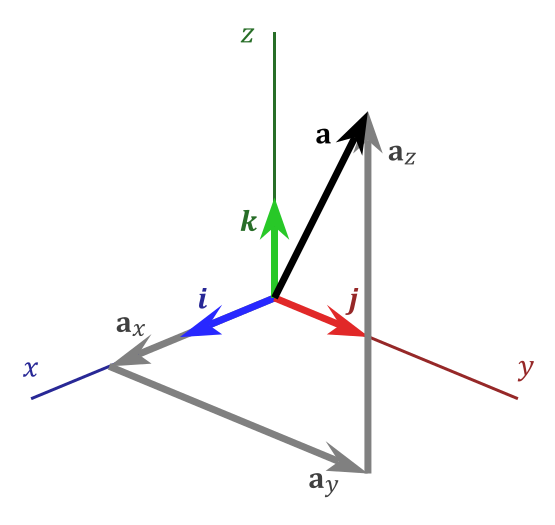
\includegraphics[width=0.5\textwidth]{3D_Vector}\label{3dS}
      La cantidad (distancia) desde el punto origen a lo largo de cada conjunto de los reales ($\mathbf{X},\mathbf{Y},\mathbf{Z}$)  
 }
\subsection{Movimiento rectilíneo uniforme}
Movimiento es que cambias de posición en un tiempo definido. Entonces la partícula está en una posición de un campo en un instante y en otra posición del campo en otra. Entonces puedes ver todos los instantes de una partícula a lo largo de una línea en un campo 3D ($\mathbb{R}^3$) o muchos campos cada uno en un instante $t$, separados por una $\dif t$-diferencial de $t$- fija infinitesimal como si $t$ fuera una dimensión más. Poniendo el primer ejemplo de la ruta de la partícula en un solo campo 3D, se puede tener al tiempo $t$ como un parámetro y graficar. Entonces el movimiento rectilíneo es el que dibuja la partícula a través de $t$ sin cambiar la dirección del movimiento, como su nombre lo indica, una línea recta. Y para que sea ese movimiento uniforme el módulo de la diferencia de posiciones entre 2 puntos de la trayectoria, debe ser igual para intervalos iguales de $t$.
Entonces para la ruta de la partícula $\mathbf{p}$ su derivada es una constante:
\begin{equation}
 \vec P(t)=\vec b+t\dif \vec p; \;
\end{equation}
en donde $\vec P(t)$ es la posición de la partícula $\mathbf{p}$ en el instante $t$  y todas las variables menos el tiempo $t$ son vectores de posición. \\
%\centering
      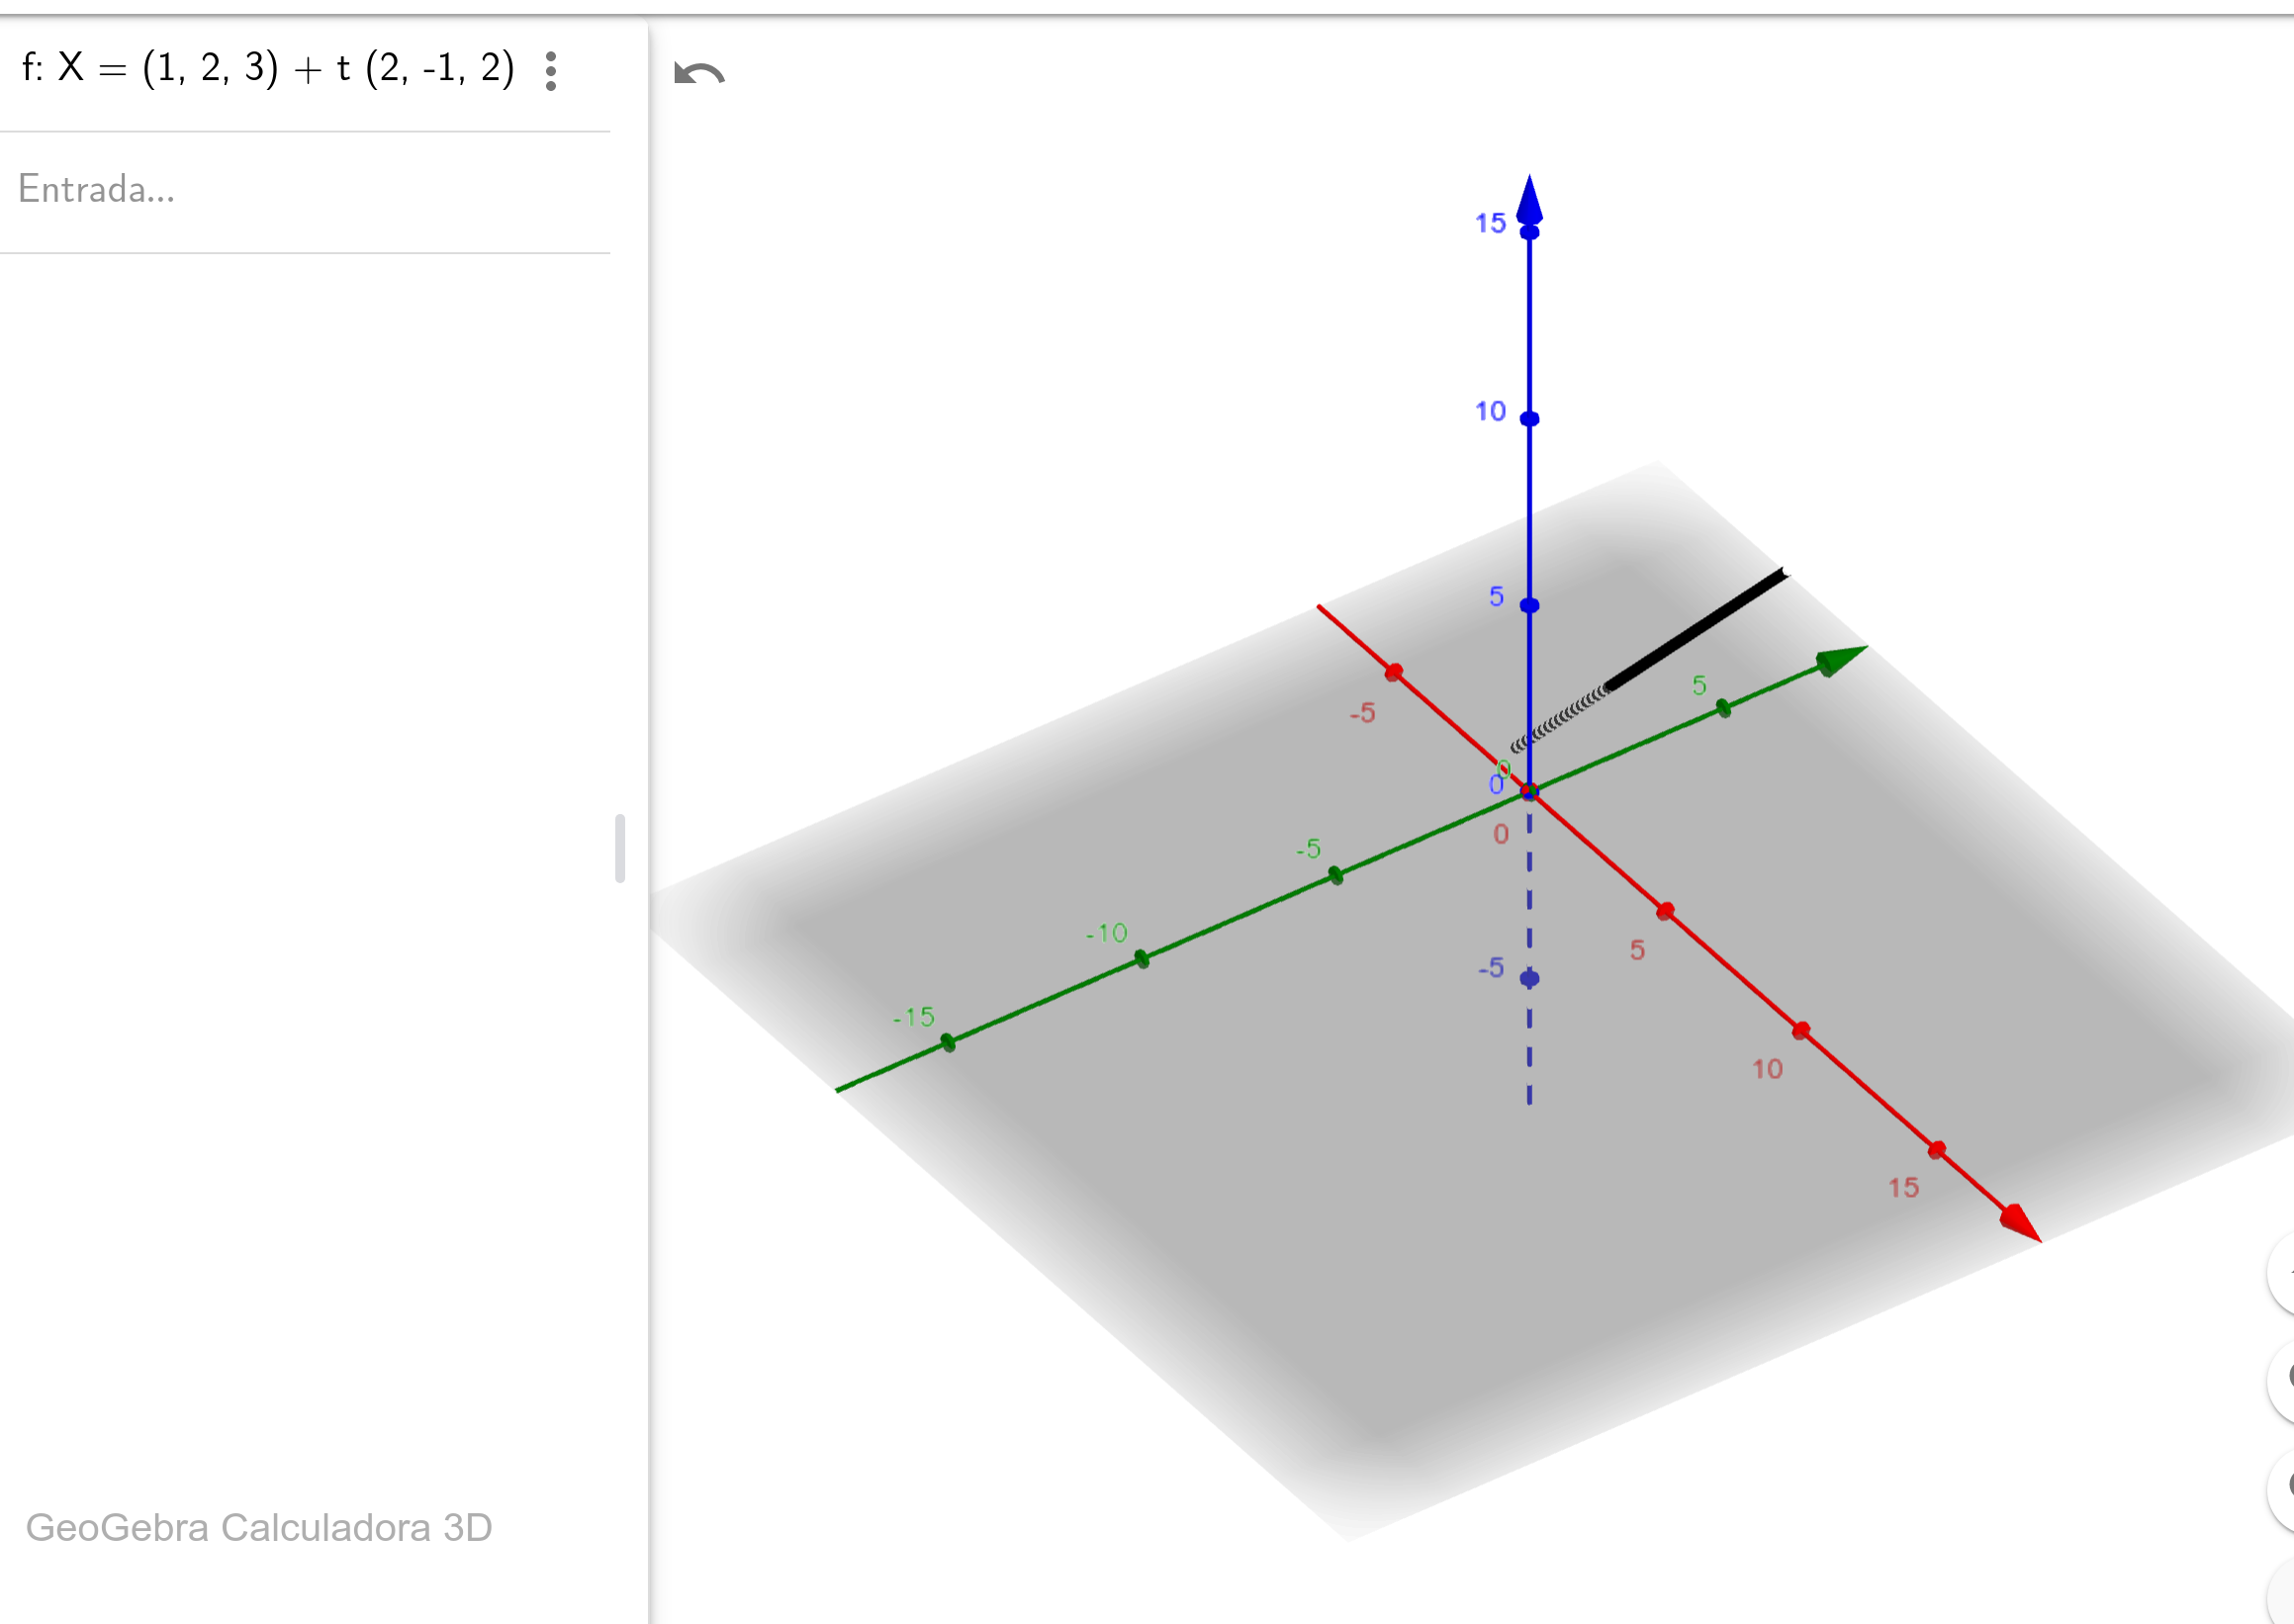
\includegraphics[width=0.9\textwidth]{MovRec}\label{rect}\\
      Movimiento rectilíneo.  
 
\subsection{Velocidad}
Velocidad es el cambio de posición para un correspondiente cambio de tiempo por lo tanto es la derivada de la posición multidimensional  con respecto al tiempo. 
\begin{equation}
 \vec V=\diff{\vec p}{t}
\end{equation}

\subsection{Aceleración}
La aceleración es el cambio de velocidad con respecto al tiempo:
\begin{equation}
 \vec A=\diff {\vec V}{t}=\diff[2]{\vec p}{t}
\end{equation}

\section{Cinética}
La Cinética estudia la relación de las fuerzas que actúan sobre un cuerpo.La cinética se usa para predecir el movimiento que van a producir ciertas fuerzas o para determinar las fuerzas necesarias para producir un cierto movimiento.
\subsection{Segunda Ley de Newton}
La segunda ley de Newton se puede formular como:
\begin{definition}
 Si la resultante de las fuerzas que actúan sobre una partícula no son cero entonces la partícula tendrá una aceleración proporcional a la magnitud y en la dirección de la resultante.
 \end{definition}
 Si nosotros tenemos una serie de fuerzas que actúan sobre una dada partícula, veremos que a mayor magnitud  fuerza sobre la partícula mayor magnitud de la aceleración de la partícula. De modo que al dividir las magnitudes de las fuerzas entre las magnitudes de las aceleraciones de la misma partícula obtendremos una constante:
 \begin{equation}
 \frac{f_1}{a_1}=\frac{f_2}{a_2}=\frac{f_3}{a_3}=\frac{f_4}{a_4}=\cdots=K
 \end{equation}
 A esa constante se le denomina masa:
 \begin{equation}
  \vec F=m\vec a
 \end{equation}
Cuando la partícula es sometida a varias fuerzas entonces la fórmula se convierte en:
\begin{equation}
 \sum \vec F=m\vec a=m\diff {\vec v}{t}
\end{equation}
donde $\sum \vec F$ es la suma o resultante de las fuerzas que se aplican a una partícula. 

Ya que la masa $m$ es una constante la suma de las fuerzas se puede expresar como:
\begin{equation}
 \sum \vec F=\diff {m \vec v}{t}
\end{equation}
a la fórmula $m\vec v$ se le conoce como momento lineal $\vec L$ (inercia) así que:
\begin{equation}
 \vec L=m\vec v \therefore\sum \vec F=\vec L'
\end{equation}
\cite{beer-statics-dynamics}
\subsection{Fricción}
Cuando se oponen 2 superficies en contacto se tiene una fuerza que se opone al deslizamiento de una por sobre la otra. A esa fuerza de oposición se le llama fricción o rozamiento.

Existen 2 tipos de fricción: fricción seca o fricción de Coulomb y fricción viscosa.

La fricción viscosa es la que los líquidos tienen entre los líquidos  y entre líguidos y sólidos. Es la que se tienen en sitios donde se usa un lubricante en la superficie de 2 sólidos para disminuir la fricción. La grasa también se considera con tipo de fricción viscosa ya que se comporta como un líquido lubricante.

Existen 2 tipos de fricción seca, la fricción estática y la fricción cinética o dinámica. 
\paragraph{La fricción estática} es la que se tiene cuando 2 superficies que no tienen movimiento entre ellas empiezan a sufrir una fuerza tangencial a sus superficies. Al principio no hay desplazamiento de una sobre la otra por lo que se va aumentando la fuerza de fricción entre ellas, no hay movimiento hasta que la fuerza tangencial entre ellas aumenta hasta un cierto punto de fuerza máxima $F_m$ llamado punto de ruptura donde un objeto empieza a desplazarse con respecto al otro y la fuerza de fricción baja drásticamente hasta la que se conoce como fuerza de fricción dinámica $F_k$. A la primera fuerza máxima en el momento de ruptura se le llama fuerza estática máxima $F_m$ y a la segunda fuerza dinámica o cinética $F_k$. Sus fórmulas son:
\begin{equation}
 F_m=\mu_s N
\end{equation}

\begin{equation}
 F_k=\mu_k N
\end{equation}

donde $N$ es la fuerza normal a la superficie de contacto y las $F_{m,k}$ son las fuerzas opuestas al movimiento y por lo tanto colineales con el mismo pero de sentido contrario y las $\mu_{s,k}$ son los coeficientes de fricción estáticos y dinámicos respectivamente.
\begin{practica}
 En una superficie plana de madera con una inclinación de 30 grados  hay una caja de cartón con 100 kg. ¿Cuál es la descomposición de las fuerzas implicadas?. ¿Cuál es el ángulo máximo antes de que la caja se empiece a deslizar?  
\end{practica}
\begin{figure}[h]
  \centering
      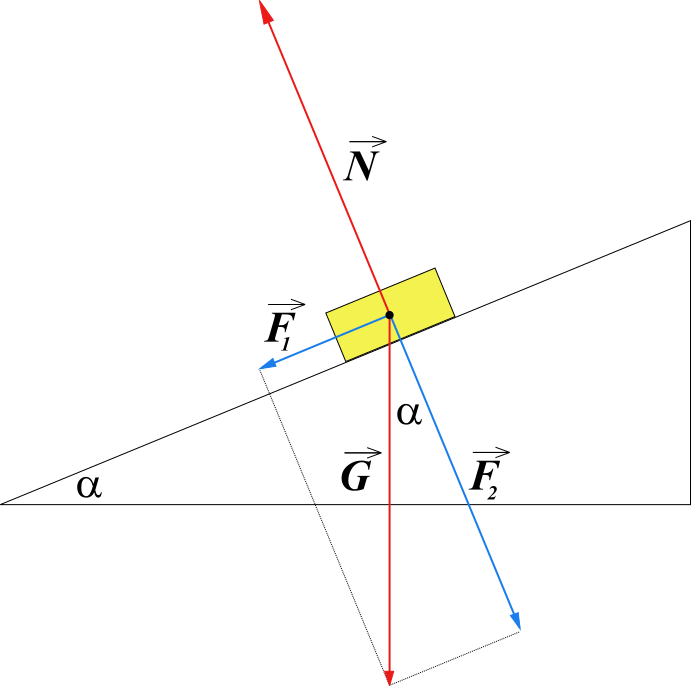
\includegraphics[width=0.5\textwidth]{Rownia}\label{MomManDer2}
  \caption{Plano inclinado.}
\end{figure}
\begin{figure}[h]
  \centering
      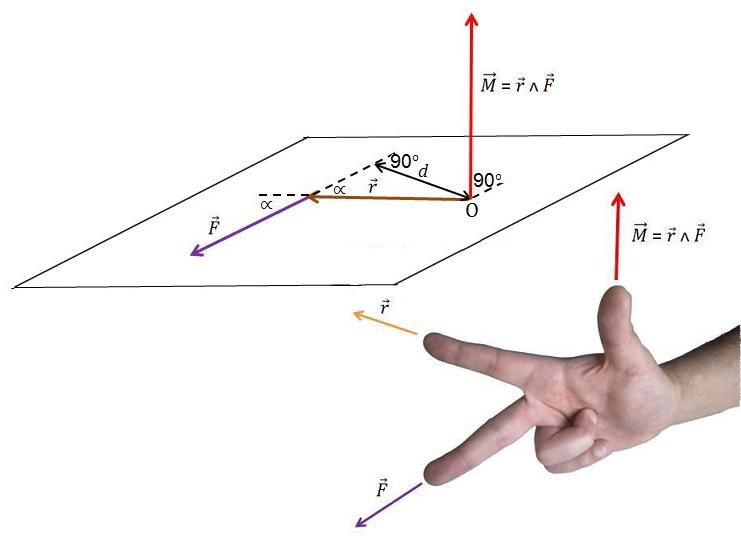
\includegraphics[width=0.5\textwidth]{regla-mano-derecha-sentido-fuerza}
  \caption{El momento cumple lar regla de la mano derecha}
\end{figure}
\cite{beer-statics-dynamics,piwiki}

\chapter{Óptica}
Como su nombre nos lo indica se trata de ver todo lo relacionado con los ojos, o sea con lo que se ve, ésto es, la energía electromagnética dentro del rango visible. 
\section{Óptica geométrica}
La óptica geométrica considera a la luz como partículas que se alejan de la fuente de luz y por lo tanto siguen una ruta recta, las líneas que trazan su ruta a partir de su origen y desviación por reflexión o refracción nos lleva a estudiar la luz desde el puento de vista de la geometría de su desplazamiento, a lo que se llama óptica geométrica.
\subsection{Concepto de luz}
 La luz es un fenómeno de naturaleza dual. Es decir se comporta como una onda y también se comporta como una partícula. Eso hace más complejo su estudio.\\
 A la luz se le conoce como lo que perciben nuestros ojos y que ilumina las cosas de modo que podemos verlas.
 Es un fenómeno electromagnético, esto es es en parte magnetismo y en parte electricidad. Cuando un campo magnético varía de intensidad provoca, perpendicularmente al mismo, un campo eléctrico y cuando un campo eléctrico cambia de posición genera un campo magnético por lo que una onda electromagnética viene a ser un campo electromagnético propagándose por el espacio o medio traslúcido a la máxima velocidad posible en ese medio , que en el caso del vacío viene a ser aproximadamente 300,000 km/s que significa que avanza  300,000 kilómetros por cada segundo que transcurre.
 
\subsection{Velocidad de la luz}
El límite de velocidad de propagación de los eventos es la velocidad de la luz. Así se llama ya que se descubrió primero con los campos electromagnéticos pero en la propagación de los campos gravitacionales también se ha visto el mismo límite.

La velocidad de propagación de la luz en el vacío es:
\begin{equation}
 c=300,000 km/s \label{c}
\end{equation}

\subsection{Reflexión y Refracción}
La luz es una onda electromagnética con frente de onda perpendicular a la propagación de la misma. Se comporta como onda y también como partícula, sin embargo no tiene masa y se desplaza a la velocidad de $c=300,000 km/s$ (ver ec. \ref{c}) .\\
La luz se desplaza en línea recta y radial al origen de la misma, de modo que sus distintas ``partículas'' llamadas fotones se separan formando una esfera que se expande a la velocidad $c$. 
\paragraph{Reflexión}
\label{sec:ref}
 es el retorno de la luz por el mismo medio en que se propagaba, al llegar a la
superficie de separación de dos sustancias distintas». Se llama ÁNGULO DE INCIDENCIA ($\varepsilon$) el
que forma el rayo incidente ($IS$) y la normal ($SN$) a la superficie. Se llama ÁNGULO DE REFLEXIÓN ($\varepsilon '$) el que forma el rayo reflejado ($SR$) y la normal ($SN$) (Fig. \ref{refl}).
\paragraph{Refracción}
\label{sec:refrac}
«es el cambio de velocidad que experimenta la luz al pasar de un medio a
otro». Este cambio de velocidad se manifiesta por una variación en la dirección de propagación, en todos los casos, excepto cuando el rayo incidente es normal a la superficie de separación de los medios. ÁNGULOS DE INCIDENCIA ($\varepsilon$) y de REFRACCIÓN ($\varepsilon '$) son los formados
por los rayos incidente ($I$) y refractado ($R$), con la normal ($N$) a la superficie en el punto de
incidencia ($S$) (Fig. \ref{refrac}).
\begin{figure}[h]
  \centering
      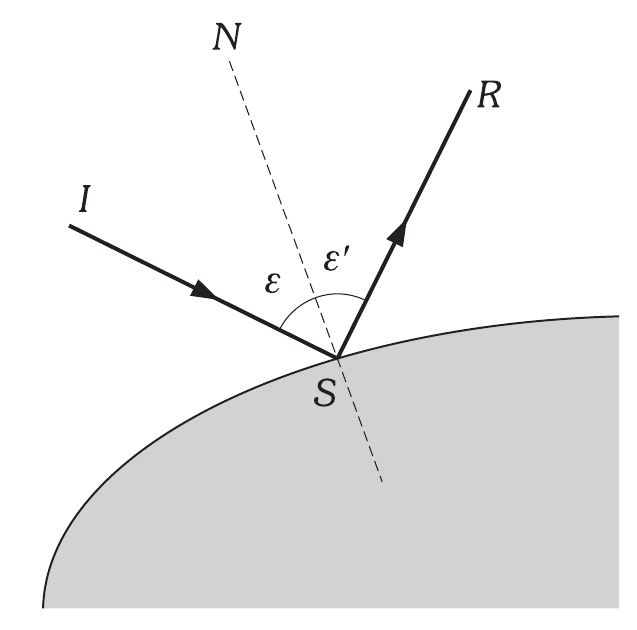
\includegraphics[width=0.5\textwidth]{Refl}
  \caption{Reflexión}\label{refl}
\end{figure}

\begin{figure}[h]
  \centering
      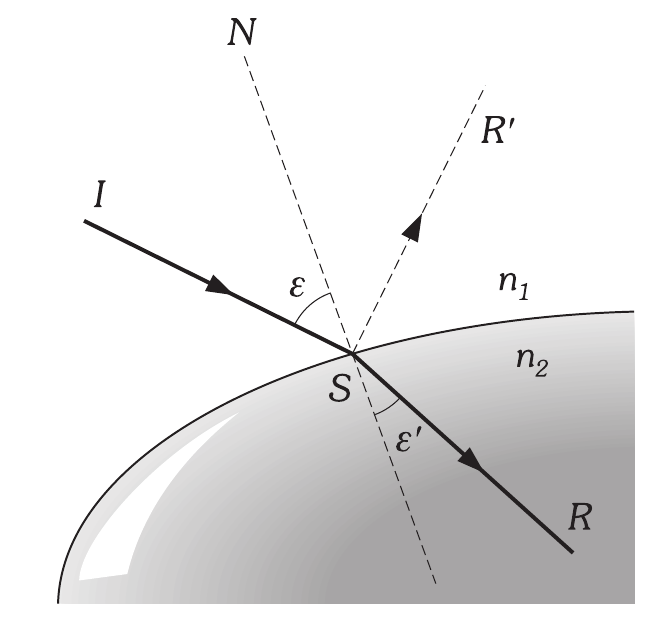
\includegraphics[width=0.5\textwidth]{Refrac}
  \caption{Refracción}\label{refrac}
\end{figure}
En las superficies refringentes la energía luminosa del rayo incidente se divide en dos, una que
corresponde al rayo refractado $R$ y otra al reflejado $R'$.
La luz viaja en los diferentes medios materiales con distinta velocidad ($v$), siempre menor con
la que lo hace en el vacío (c). Ópticamente se caracterizan los medios transparentes por un escalar
($n$) que se define como:
\begin{equation}
 n=\frac{c}{v}
\end{equation}
llamado índice de refracción absoluto de una substancia. $n$ es siempre mayor que la unidad, puesto que $v$ es siempre menor que $c$. (El índice de refracción del aire
se puede considerar la unidad, ya que su valor es 1.000 293).

Para los cálculos de las trayectorias de los rayos de luz en el caso de reflexión (fig. \ref{refl}), el ángulo de incidencia es igual al ángulo del rayo reflejado:
\begin{equation}
 \varepsilon=\varepsilon '
\end{equation}
Para el cálculo de los rayos refractados (fig. \ref{refrac}) la relación entre los ángulos es la siguiente:
\begin{equation}
 n \sen(\varepsilon)=n' \sen(\varepsilon ')
\end{equation}

\cite{burbano}´
\subsection{Fibra óptica}
\paragraph{Ángulo límite}
\label{sec:angLím} es el ángulo de incidencia que corresponde a uno de refracción de 90\textdegree
Al rayo $A$ (normal) (Fig. \ref{anglim}) corresponde el refractado $A'$ (normal); al $B$ el $B'$, apartado
de la normal más que el incidente; a $C$ el $C'$ rasante a la superficie. El ángulo de incidencia $l$, al
que corresponde el refractado.
 Al ángulo de la trayectoria $A'SC$ = 90\textdegree , se le llama el ángulo límite.\\
 A un rayo $D$ que incide con ángulo mayor que el límite no corresponde rayo refractado, reflejándose en la superficie de separación de los dos medios y verificando el fenómeno de la reflexión total, llamado así porque toda la intensidad del rayo incidente la contiene el rayo reflejado, a
diferencia de los rayos que inciden con ángulo igual o menor que el límite ($B$) cuya intensidad se
reparte entre el refractado ($B'$) y el reflejado ($B''$), de puntos en la figura.\\
\begin{figure}[h]
  \centering
      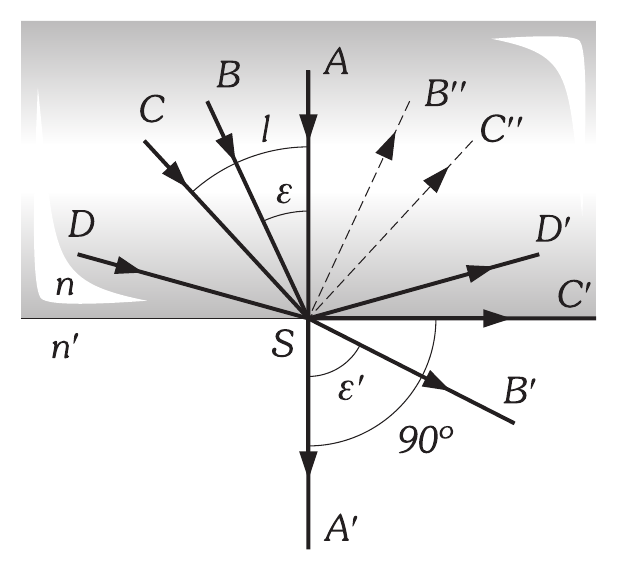
\includegraphics[width=0.5\textwidth]{AngLim}
  \caption{Ángulo límite}\label{anglim}
\end{figure}

Para que se verifique el fenómeno de la REFLEXIÓN TOTAL son necesarios dos condiciones:
que la luz vaya en un medio más hacia otro menos refringente y que incida con un ángulo
mayor que el límite. Entonces el ángulo límite para que haya reflexión total es:
\begin{equation}
 n\sen \varepsilon=n'\Rightarrow \varepsilon=\sen^{-1}\left(\frac{n'}{n}\right)
\end{equation}


La fibra óptica es una de las muchas aplicaciones de la reflexión total; se fabrican con vidrios y plásticos
de alto índice de refracción y de un diámetro de unos pocos micrómetros. La Fig. \ref{fibra} nos
hace comprender su fundamento; la luz, penetra normalmente a la superficie extrema plana, quedando atrapada en su interior el rayo incidente, en sus múltiples reflexiones con las paredes. Sufriendo el fenómeno de reflexión total, hasta salir por el otro extremo de la fibra. La fibra óptica puede usarse para transmitir luz codificada con señales digitales, rodeando obstáculos y a distancias muy largas casi
sin pérdidas; en su formación debe, cada fibra, aislarse ópticamente, mediante un recubrimiento
muy fino de un material cuyo índice de refracción sea menor que el de la fibra interna y una capa opaca al exterior para que no penetre luz externa que pueda interferir con los datos transmitidos.
\begin{figure}[h]
  \centering
      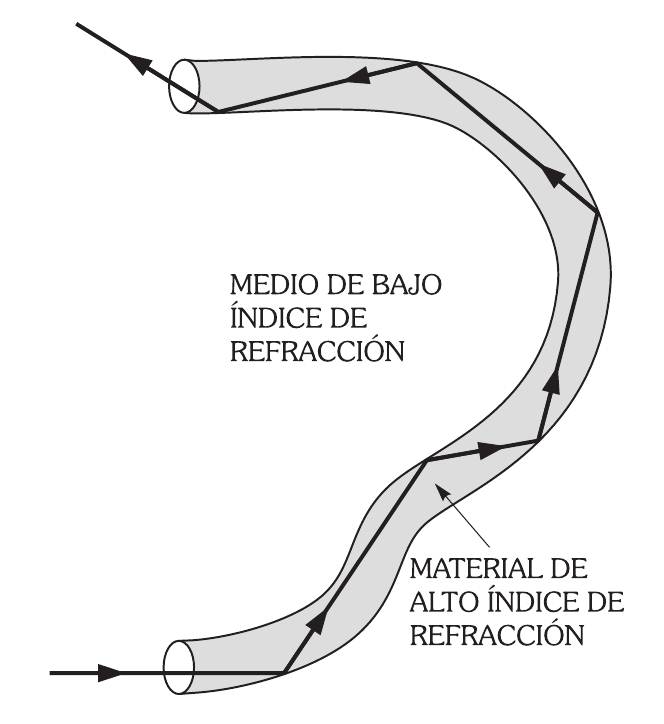
\includegraphics[width=0.5\textwidth]{Fibra}
  \caption{Fibra óptica}\label{fibra}
\end{figure}


\cite{burbano}

\subsection{Lentes}
La forma esférica o curva de las superficies de medios transparentes, puede servir por refracción para cambiar la dirección del flujo común de la luz. A ciertos dispositivos que desvían el flujo de la luz se les conoce como lentes de refracción. 
Los lentes se usan para concentrar o expander el flujo de la luz, ampliar o achicar las imágenes  de allí su nombre convergentes o divergentes (ver fig. \ref{lentes}).
\begin{figure}[h]
  \centering
      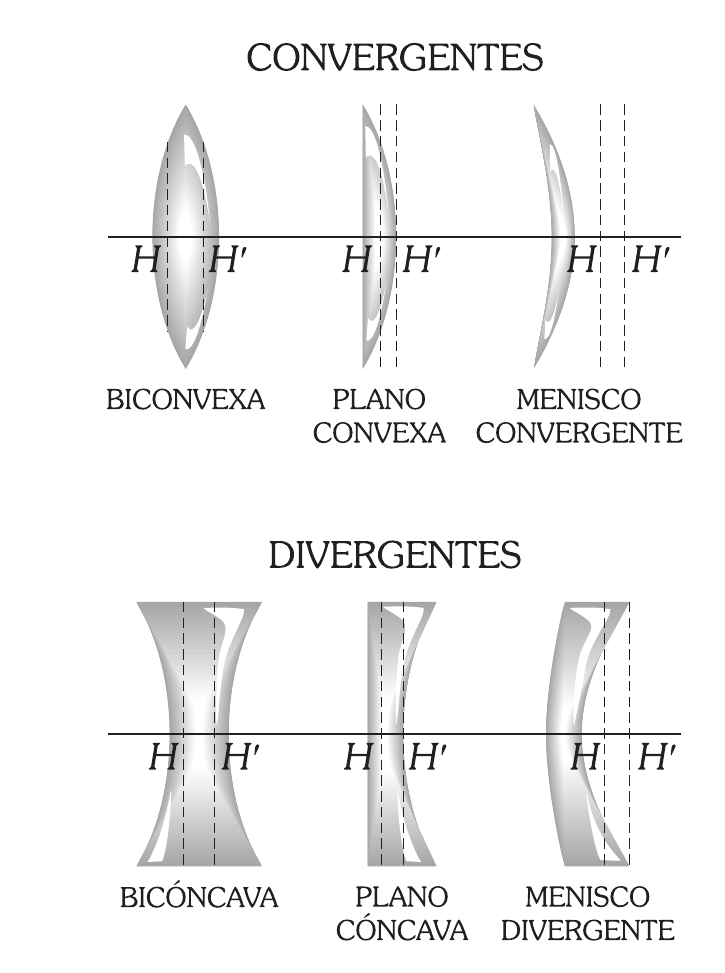
\includegraphics[width=0.5\textwidth]{lentes.png}
  \caption{Lentes convergentes y lentes divergentes}\label{lentes}
\end{figure}
Con los lentes convergentes se obtiene una imagen virtual invertida de los objetos que se encuentren del otro lado del lente, por eso los lentes nos sirven para crear imágenes en cámaras de fotos, cámaras de videos, telescopios, binoculares, etc.. Incluso nuestros ojos tienen un lente llamado cristalino que genera una imagen invertida en el fondo ocular que es transmitida a nuestro cerebro para que el mismo interprete la forma del mundo a nuestro alrededor.

A la distancia donde el lente genera una imagen invertida de objetos lejanos se le conoce como distancia focal o simplemente $f$ del lente. A mayor $f$ del lente mayor la imagen generada. Nuestros ojos generan en nuestro cerebro una imagen aproximada al $f=50\rightarrow 55 mm$

Los lentes se usan en computadoras para cámaras web y de video, entrada y salida de la luz en la fibra óptica, en los lectores de CDs, DVDs y Bluerays, etc.
\cite{burbano}
\subsection{El telescopio}
Si se aumenta la distancia focal de un lente, la imagen virtual generada puede ser aumentada con un lente o lentes adicionales. El dispositivo con distancia focal mayor a $500 mm$ se le conoce como telescopio. En general tiene 2 lentes, un lente llamado objetivo que está más cercano al objeto que se va a estudiar y el lente ocular que aumenta la imagen generada por el lente objetivo.
\section{Estudio y aplicaciones de emisión láser}
La palabra láser es un acrónimo que significa Light Amplified by Stimulated Emission of Radiation (Luz amplificada por emisión estimulada de radiación). Un láser es básicamente una fuente de luz. Lo que diferencia a un láser de otras fuentes de luz, como las bombillas, es el mecanismo físico por el que se produce la emisión de luz, que se basa en la emisión estimulada, en contra de la emisión espontánea que es la responsable de la mayor parte de la luz que vemos. Para entender lo que es la emisión espontánea y la emisión estimulada hay que conocer un poco la física de la interación de átomos con fotones. Tan solo diremos aquí que este particular mecanismo de emisión confiere a la luz unas propiedades muy interesantes, como son la alta potencia (y su capacidad para ser amplicada), la direccionalidad (emsión en forma de “rayos”), la frecuencia de emisión bien definida (colo de la luz), la capacidad de emitirse en pulsos de muy corta duración, y una propiedad llamada coherencia que significa que las onda electromagnéticas que forma el haz de luz marchan “al paso”.

\paragraph{Monocromaticidad.}
\label{sec:monocromaticidad}
Emite una radiación electromagnética de una sola longitud de onda, en oposición a las fuentes convencionales como las lámparas incandescentes (bombillas comunes) que emiten en un rango más amplio, entre el visible y el infrarrojo, de ahí que desprendan calor. La longitud de onda, en el rango del espectro electromagnético de la luz visible, se identifica por los diferentes colores (rojo, naranja, amarillo, verde, azul, violeta), estando la luz blanca compuesta por todos ellos. Esto se observa fácilmente al hacer pasar un haz de luz blanca a través de un prisma.

\paragraph{Coherencia espacial o direccionabilidad.}
La radiación láser tiene una divergencia muy pequeña, es decir, puede ser proyectado a largas distancias sin que el haz se abra o disemine la misma cantidad de energía en un área mayor.

Nota: Esta propiedad se utilizó para calcular la longitud entre la Tierra y la Luna, al enviar un haz láser hacia la Luna, donde rebotó sobre un pequeño espejo situado en su superficie, y éste fue medido en la Tierra por un telescopio.

\paragraph{Coherencia temporal.} La luz láser se transmite de modo paralelo en una única dirección debido a su naturaleza de radiación estimulada, al estar constituido el haz láser con rayos de la misma fase, frecuencia y amplitud.

\paragraph{Las aplicaciones del láser más cotidianas de los sistemas de computación son:}, el lector del código de barras, el almacenamiento óptico y la lectura de información digital en discos compactos (CD) o en discos versátiles digitales (DVD) u Bluray, que se diferencían los primeros de los últimos en que éstos últimos utilizan una longitud de onda más corta (emplean láser azul en vez de rojo). Otra de las aplicaciones son las fotocopiadoras e impresoras láser, o las comunicaciones mediante fibra óptica. Las aplicaciones para un futuro próximo son los ordenadores cuánticos u ópticos que serán capaces de procesar la información a la velocidad de la luz al ir los impulsos eléctricos por pulsos de luz proporcionados por sistemas láser. También se usa el rayo láser en muchos de los procesos de fabricación de los componentes electrónicos que tienen en su estructura las computadoras, como por ejemplo resistencias, en las cuales es necesario volatilizar muy pequeñas cantidades de material para fabricar resistencias de muy alta precisión.
\cite{laser}
\chapter{Introducción a la Termodinámica}
\section{Definiciones}
\section{Escalas de temperatura}
\section{Capacidad calorífica}
\section{Leyes de la Termodinámica}
\chapter{Electrostática}
\section{Definiciones}
\section{Sistemas de unidades}
\section{Carga eléctrica y sus propiedades}
\section{Leyes de la electrostática}
\section{Campo eléctrico}
\section{Cálculo de potencial eléctrico en diferentes configuraciones}
\section{Capacitores con dieléctrico}
\section{Energía asociada a un campo eléctrico}
\section{Capacitores en serie y paralelo}
\chapter{Electrodinámica}
\section{Definiciones de corriente, resistencia,
resistividad, densidad de corriente y
conductividad}
\section{Ley de Ohm}
\section{Potencia}
\section{Leyes de Kirchhoff}

\chapter{Electromagnetismo}
\section{Definiciones}
\section{Campo magnético terrestre}
\section{Trayectoria de las cargas en movimiento dentro de un campo magnético}
\section{Fuerzas magnéticas entre corrientes}
\section{Leyes de electromagnetismo}
\section{Ley de Ampere}
\section{Inductancia magnética}
\section{Energía asociada con un campo magnético}
\section{Densidad de energía magnética}
\section{Aplicaciones}



%\bibliographystyle{plain}
%\bibliography{EDA-biblio} 





\printbibliography[heading=bibintoc]



\end{document}

